\section{Schlauchbeutelmaschine}
Mit diesem Beispiel kann man die bestehende Architektur durch eine weitere Maschine ergänzen. Es ist problemlos möglich
auch Weitere oder andere Maschinen oder Module einer Maschine einzurichten. Allerdings soll mit diesem Beispiel die
allgemeine Vorgehensweise erklärt werden.

In Abbildung~\ref{fig:siegelmaschinen_vffs} auf Seite~\pageref{fig:siegelmaschinen_vffs} ist der schematische Aufbau der
vertikalen Schlauchbeutelmaschine aufgezeigt.

\begin{figure}[h]
    \centering
    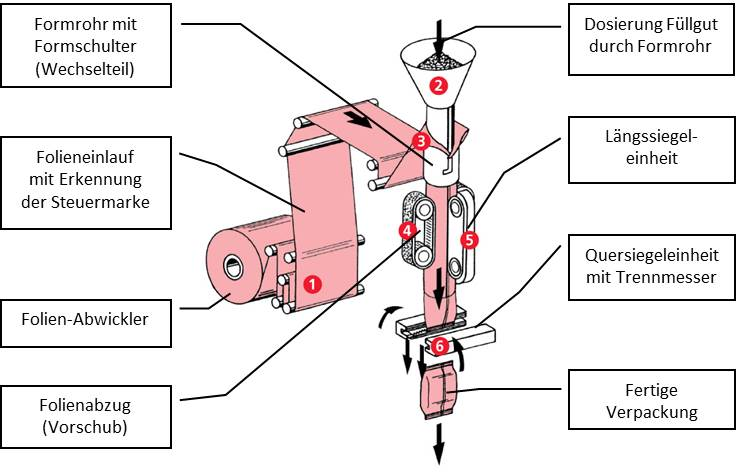
\includegraphics[scale=1]{images/kapitel_5/vffs.jpg}
    \caption{Aufbau einer vertikalen Schlauchbeutelmaschine~\cite{online_grundlagen_boschkwe}}
    \label{fig:siegelmaschinen_vffs}
\end{figure}

Dort ist gut zu sehen, dass in der Abbildung im oberen Bereich unter der Nummer 2 das zu befüllende Produkt einlegt
wird. Dies fällt dann durch das Rohr bei Nummer 3. Die Folie umschließt das Produkt anschließend und wird mit den
Siegelbacken (Nummer 5) geschlossen. Bei Nummer 6 wird der befüllte Beutel von der Endlosfolie abgetrennt und kann
weiter verarbeitet werden.

Die wichtigsten Einstellparameter der Maschine betreffen die Siegelung der Folie. Da es zahlreiche Folienarten von
verschiedenen Anbietern existieren ist es nicht immer einfach, die Folie richtig zu versiegeln.

Die \textit{Siegelnahtfestigkeit} gibt an, welche Kraft notwendig ist, um die Siegelnaht wieder zu öffnen. Dies ist
insbesondere dann Wichtig, wenn es sich bei dem verpackten Produkt um ein Endkunden-Produkt handelt. Der Käufer sollte
dies unter normalem Kraftaufwand öffnen können, damit er an das Produkt gelangen kann.

Allerdings darf die Siegelnaht nicht zu schwach sein, da sonst Luft oder andere Gase in die Verpackung eindringen
könnten. Für die vertikalen Schlauchbeutelmaschine ist es entscheidend die richtige Siegelnahtfestigkeit zu erzeugen.

Zur Erzeugung einer Siegelnaht sind Daten zur \textit{Siegeltemperatur}, \textit{Siegelzeit} und \textit{Folienart}
interessant. Bei der Folie spielt der Aufbau der Folie (anzahl der Lagen, genutzte Materialien) eine Rolle.

Der genaue Aufbau von Folien wird von den entsprechenden Herstellern oft geheim gehalten und man muss ihn entweder
händisch ermitteln oder auf Erfahrungen von Mitarbeitern zurückgreifen.

Aus diversen Tests kann man anhand der eingestellten Parameter für Siegeltemperatur und Siegelzeit und der genutzten
Folie die Siegelnahtfestigkeiten ableiten, indem man den Kraftaufwand zum öffnen der Siegelnaht misst.

\subsection{Daten zusammenstellen}
Um an Testdaten für das Aufbauen eines neuronalen Netzes für diesen Maschinentyp zu kommen, sind zahlreiche Tests und
Versuche notwendig.

Für die Versuche muss man verschiedene Temperaturen mit verschiedenen Siegelzeiten mit verschiedenen Folien kreuzen, was
einen enormen Zeitaufwand bedeutet, da man jede erzeugte Siegelnaht mit Hilfe einer anderen Maschine prüfen und
auswerten muss.

Diese Maschine gibt die benötigte Kraft an, um die erzeugte Siegelnaht zu öffnen und ist normiert. Dies ist wichtig um
keine subjektive Komponente miteinzubauen (\enquote{Die war nun Fester als die davor}).

Herr Felix Kruppa von der Robert Bosch GmbH hat während seiner Dissertation einen Siegelteststand aufgebaut, welcher
verschiedene Siegelnähte erzeugen kann.

Für den Aufbau seines Teststandes durchlief er zahlreiche Tests, welche er mit einem Protokoll dokumentierte. Diese
Daten können für die Erstellung des neuronalen Netzes fungieren, da er ebenfalls die resultierende Siegelnahtfestigkeit
ermittelte und festhielt.

In Abbildung~\ref{fig:siegelmaschinen_vffs_simulator} auf Seite~\pageref{fig:siegelmaschinen_vffs_simulator} ist der
aufgebaute Siegelteststand mit seiner Beschreibung zu sehen.

\begin{figure}[h]
    \centering
    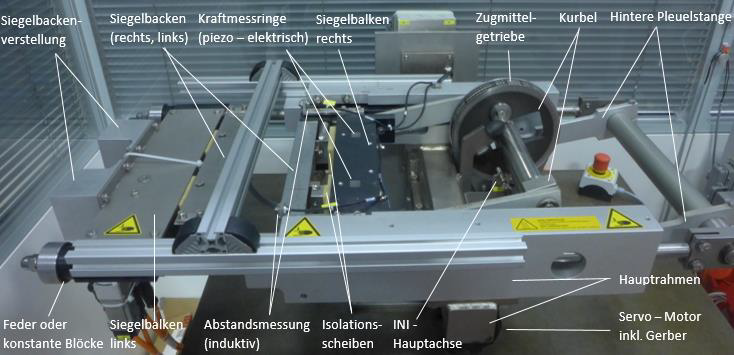
\includegraphics[width=\textwidth]{images/kapitel_5/vffs_simulator.png}
    \caption{Aufbau Siegelteststand}
    \label{fig:siegelmaschinen_vffs_simulator}
\end{figure}

Die kombinierten Daten aus den Testdurchläufen von Herrn Felix Kruppa sind im Anhang~\ref{sec:schlauchbeutelmaschine}
auf Seite~\pageref{sec:schlauchbeutelmaschine} zu sehen und man kann diese direkt für das Trainieren des neuronalen
Netzes nutzen.

%% TODO noch schreiben
\subsection{Neuronales Netz trainieren}
Hier kommt was
\colorbox{yellow}{Hier fehlt was}

%% TODO noch schreiben
\subsection{Deployment erstellen}
Hier kommt was
\colorbox{yellow}{Hier fehlt was}

%% TODO noch schreiben
\subsection{API Connect erweitern}
Hier kommt was
\colorbox{yellow}{Hier fehlt was}

%% TODO noch schreiben
\subsection{Frontend erweitern}
Hier kommt was
\colorbox{yellow}{Hier fehlt was}